\documentclass[11pt]{article}
\usepackage[textwidth=18.0cm, textheight=23.0cm, top=2.0cm]{geometry}
\usepackage{pst-all}
\usepackage{amssymb}
\usepackage{tikz}
\usepackage{underscore}\begin{document}
\pagestyle{empty}


ClassName: \underline{\textbf{Class_07.2bp-0}}
\par
BinSize: \underline{\textbf{100 × 100}}
\par
ReduceSize: \underline{\textbf{100 × 100}}
\par
TypeNum: \underline{\textbf{20}}
\par
Num: \underline{\textbf{20}}
\par
OutS: \underline{\textbf{50000}}
\par
InS: \underline{\textbf{43863}}
\par
Rate: \underline{\textbf{0.877}}
\par
UB: \underline{\textbf{5}}
\par
LB0: \underline{\textbf{5}}
\par
LB: \underline{\textbf{5}}
\par
LBWithCut: \underline{\textbf{5}}
\par
NodeCut: \underline{\textbf{0}}
\par
ExtendedNodeCnt: \underline{\textbf{1}}
\par
GenNodeCnt: \underline{\textbf{1}}
\par
PrimalNode: \underline{\textbf{0}}
\par
ColumnCount: \underline{\textbf{5}}
\par
TotalCutCount: \underline{\textbf{0}}
\par
RootCutCount: \underline{\textbf{0}}
\par
LPSolverCnt: \underline{\textbf{1}}
\par
PricingSolverCnt: \underline{\textbf{0}}
\par
BranchAndBoundNum: \underline{\textbf{1}}
\par
isOpt: \underline{\textbf{true}}
\par
TimeOnInitSolution: \underline{\textbf{0.010 s}}
\par
TimeOnPrimal: \underline{\textbf{0.000 s}}
\par
TimeOnPricing: \underline{\textbf{0.000 s}}
\par
TimeOnRmp: \underline{\textbf{0.090 s}}
\par
TotalTime: \underline{\textbf{0.165 s}}
\par
\newpage


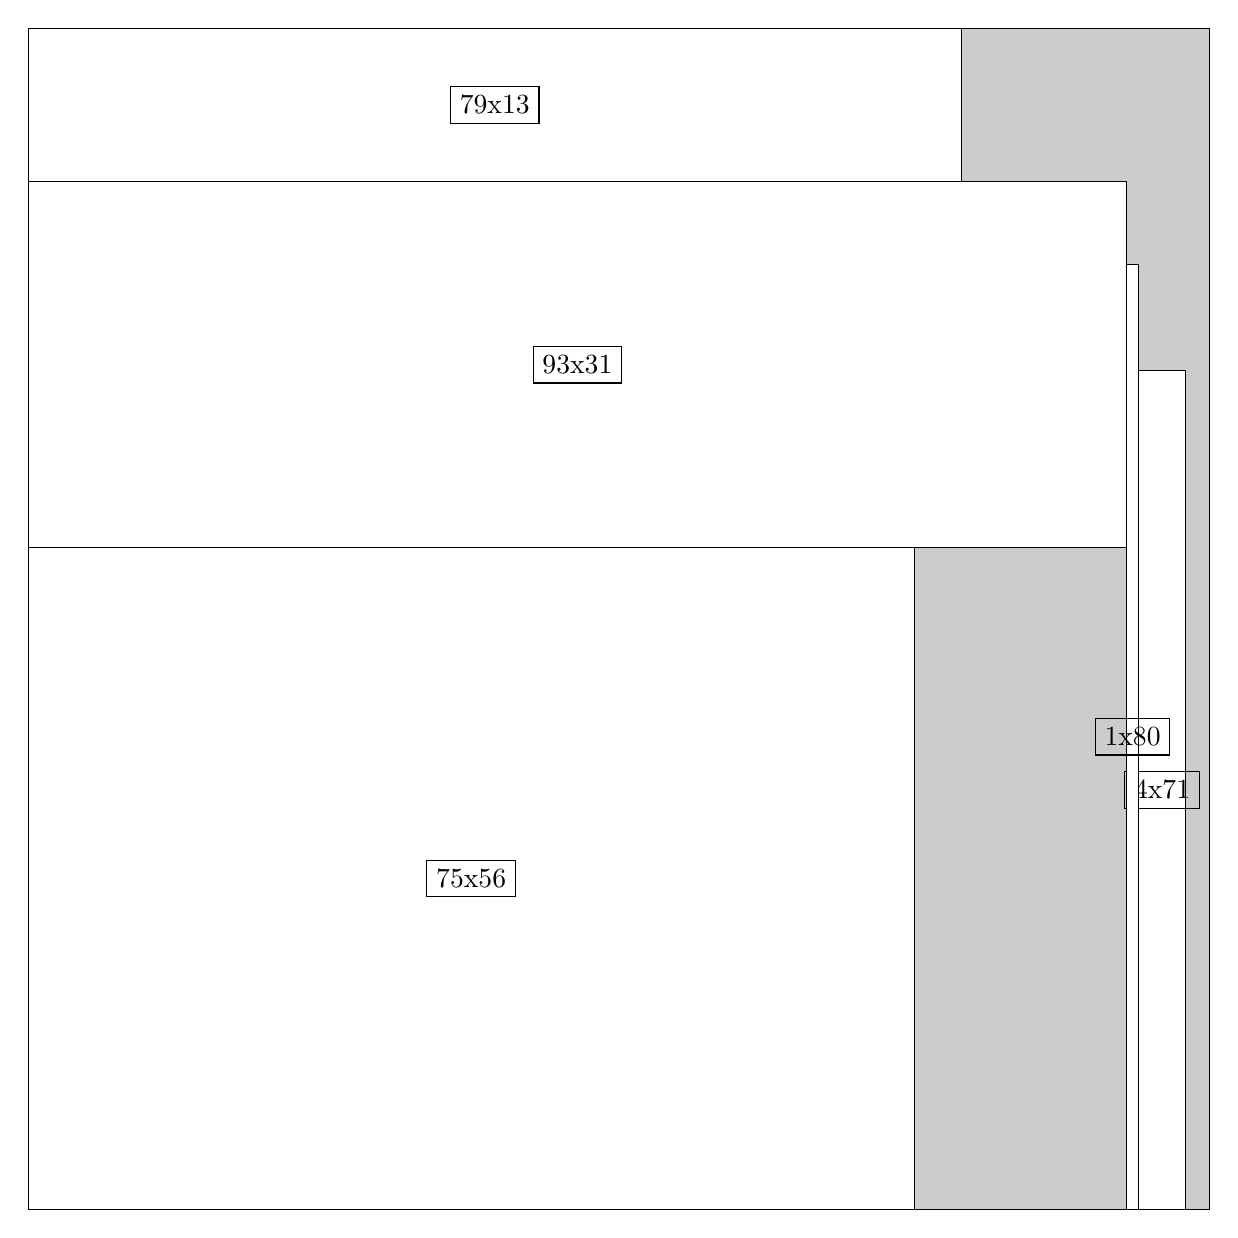
\begin{tikzpicture}[shorten >=1pt,scale=1.0,every node/.style={scale=1.0},->]
\tikzstyle{vertex}=[circle,fill=black!25,minimum size=14pt,inner sep=0pt]
\filldraw[fill=gray!40!white, draw=black] (0,0) rectangle (15.0,15.0);
\foreach \name/\x/\y/\w/\h in {75x56/0.0/0.0/11.25/8.4,93x31/0.0/8.4/13.95/4.6499999999999995,79x13/0.0/13.049999999999999/11.85/1.95,4x71/14.1/0.0/0.6/10.65,1x80/13.95/0.0/0.15/12.0}
\filldraw[fill=white!40!white, draw=black] (\x,\y) rectangle node[draw] (\name) {\name} ++(\w,\h);
\end{tikzpicture}


w =75 , h =56 , x =0 , y =0 , v =4200
\par
w =93 , h =31 , x =0 , y =56 , v =2883
\par
w =79 , h =13 , x =0 , y =87 , v =1027
\par
w =4 , h =71 , x =94 , y =0 , v =284
\par
w =1 , h =80 , x =93 , y =0 , v =80
\par
\newpage


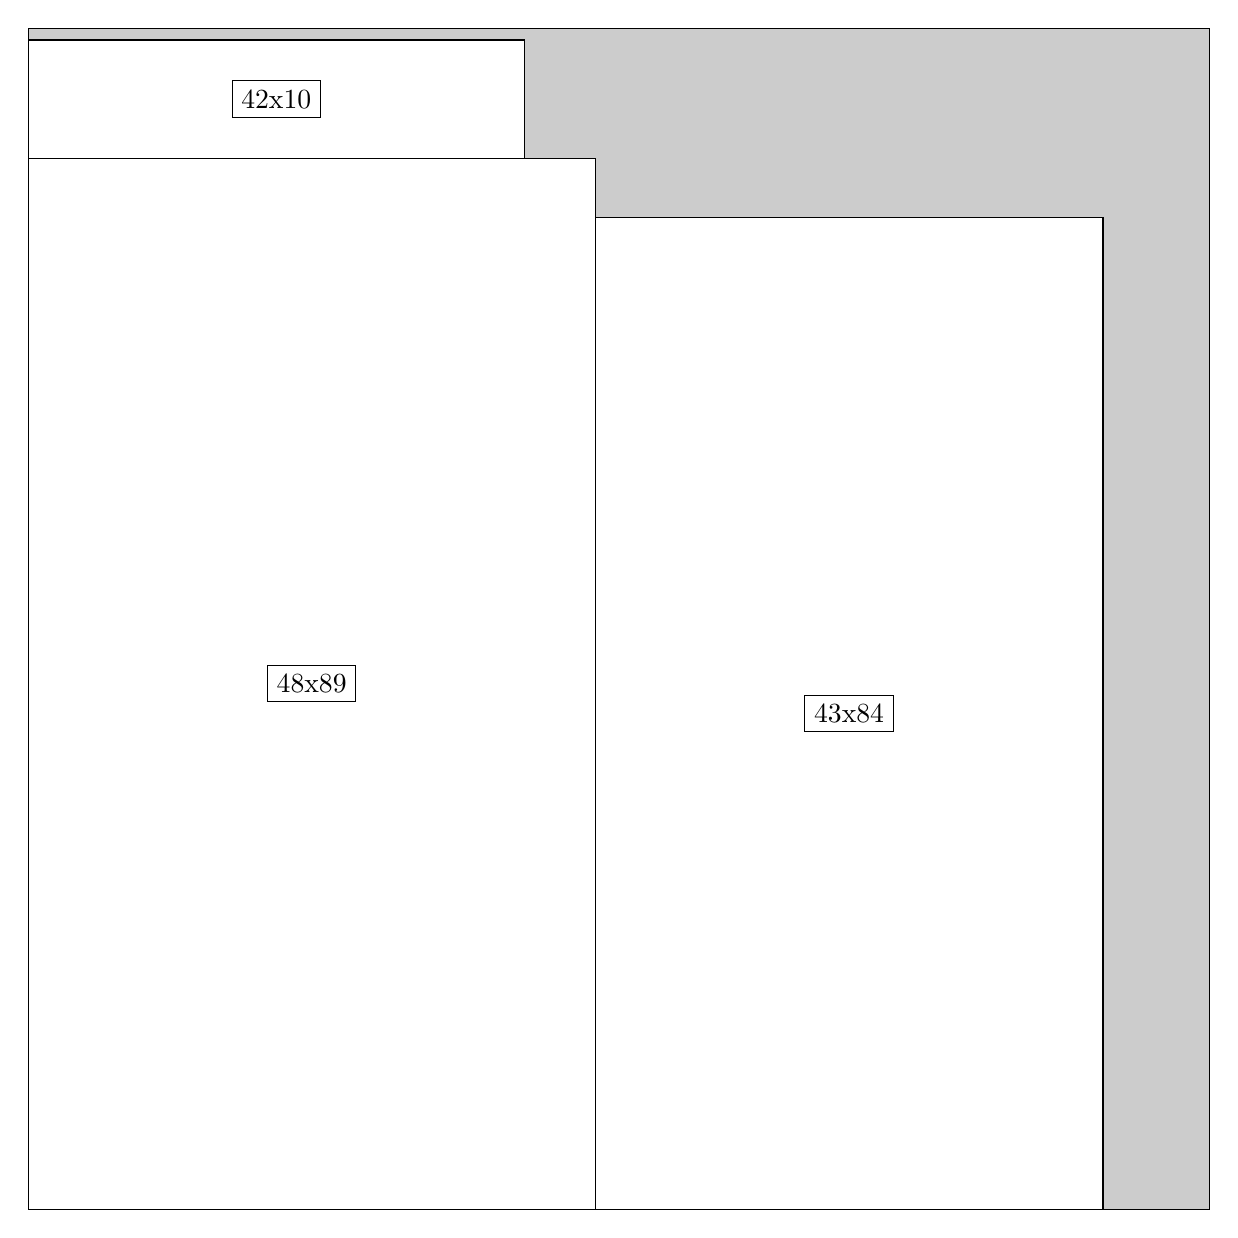
\begin{tikzpicture}[shorten >=1pt,scale=1.0,every node/.style={scale=1.0},->]
\tikzstyle{vertex}=[circle,fill=black!25,minimum size=14pt,inner sep=0pt]
\filldraw[fill=gray!40!white, draw=black] (0,0) rectangle (15.0,15.0);
\foreach \name/\x/\y/\w/\h in {48x89/0.0/0.0/7.199999999999999/13.35,43x84/7.199999999999999/0.0/6.45/12.6,42x10/0.0/13.35/6.3/1.5}
\filldraw[fill=white!40!white, draw=black] (\x,\y) rectangle node[draw] (\name) {\name} ++(\w,\h);
\end{tikzpicture}


w =48 , h =89 , x =0 , y =0 , v =4272
\par
w =43 , h =84 , x =48 , y =0 , v =3612
\par
w =42 , h =10 , x =0 , y =89 , v =420
\par
\newpage


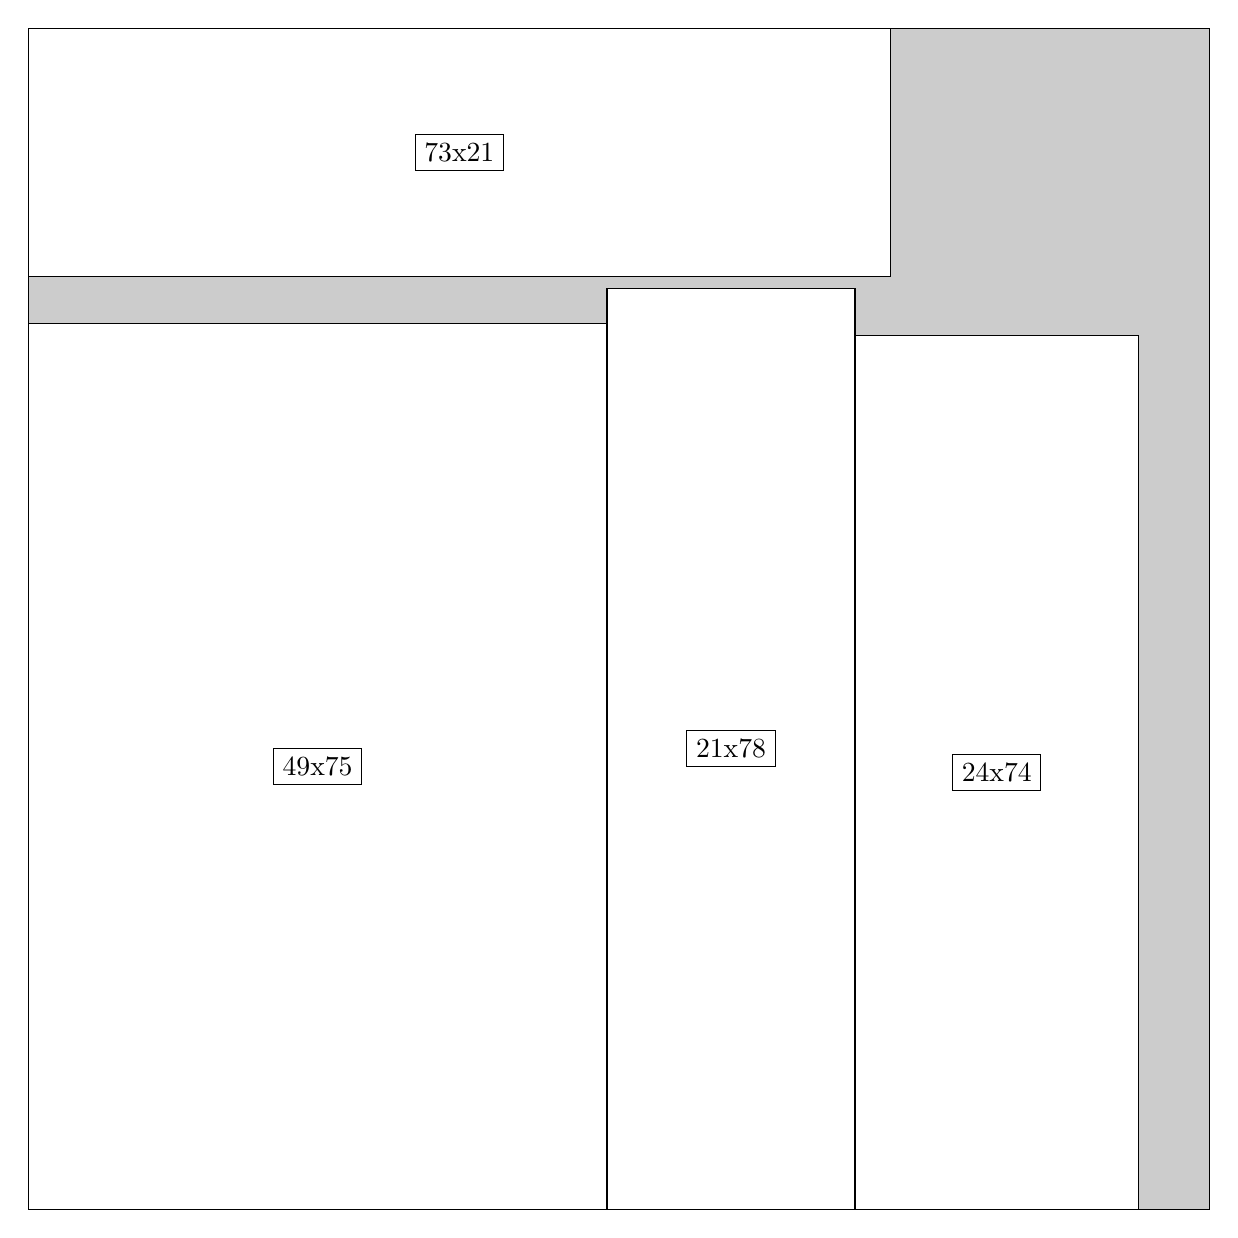
\begin{tikzpicture}[shorten >=1pt,scale=1.0,every node/.style={scale=1.0},->]
\tikzstyle{vertex}=[circle,fill=black!25,minimum size=14pt,inner sep=0pt]
\filldraw[fill=gray!40!white, draw=black] (0,0) rectangle (15.0,15.0);
\foreach \name/\x/\y/\w/\h in {49x75/0.0/0.0/7.35/11.25,24x74/10.5/0.0/3.5999999999999996/11.1,21x78/7.35/0.0/3.15/11.7,73x21/0.0/11.85/10.95/3.15}
\filldraw[fill=white!40!white, draw=black] (\x,\y) rectangle node[draw] (\name) {\name} ++(\w,\h);
\end{tikzpicture}


w =49 , h =75 , x =0 , y =0 , v =3675
\par
w =24 , h =74 , x =70 , y =0 , v =1776
\par
w =21 , h =78 , x =49 , y =0 , v =1638
\par
w =73 , h =21 , x =0 , y =79 , v =1533
\par
\newpage


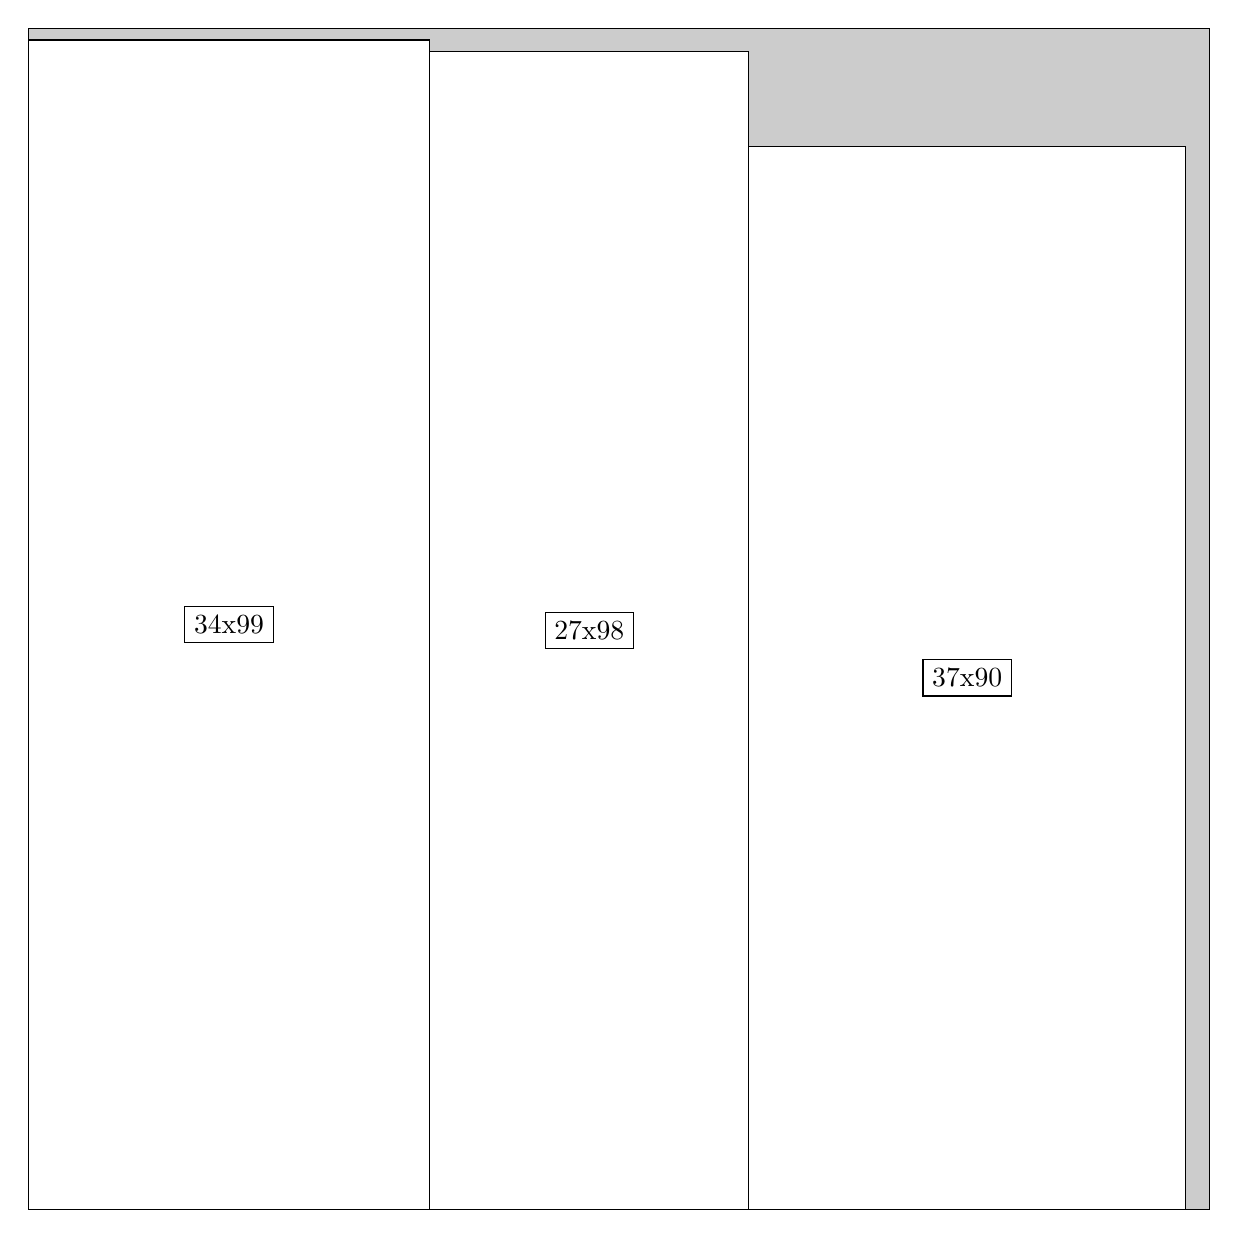
\begin{tikzpicture}[shorten >=1pt,scale=1.0,every node/.style={scale=1.0},->]
\tikzstyle{vertex}=[circle,fill=black!25,minimum size=14pt,inner sep=0pt]
\filldraw[fill=gray!40!white, draw=black] (0,0) rectangle (15.0,15.0);
\foreach \name/\x/\y/\w/\h in {34x99/0.0/0.0/5.1/14.85,37x90/9.15/0.0/5.55/13.5,27x98/5.1/0.0/4.05/14.7}
\filldraw[fill=white!40!white, draw=black] (\x,\y) rectangle node[draw] (\name) {\name} ++(\w,\h);
\end{tikzpicture}


w =34 , h =99 , x =0 , y =0 , v =3366
\par
w =37 , h =90 , x =61 , y =0 , v =3330
\par
w =27 , h =98 , x =34 , y =0 , v =2646
\par
\newpage


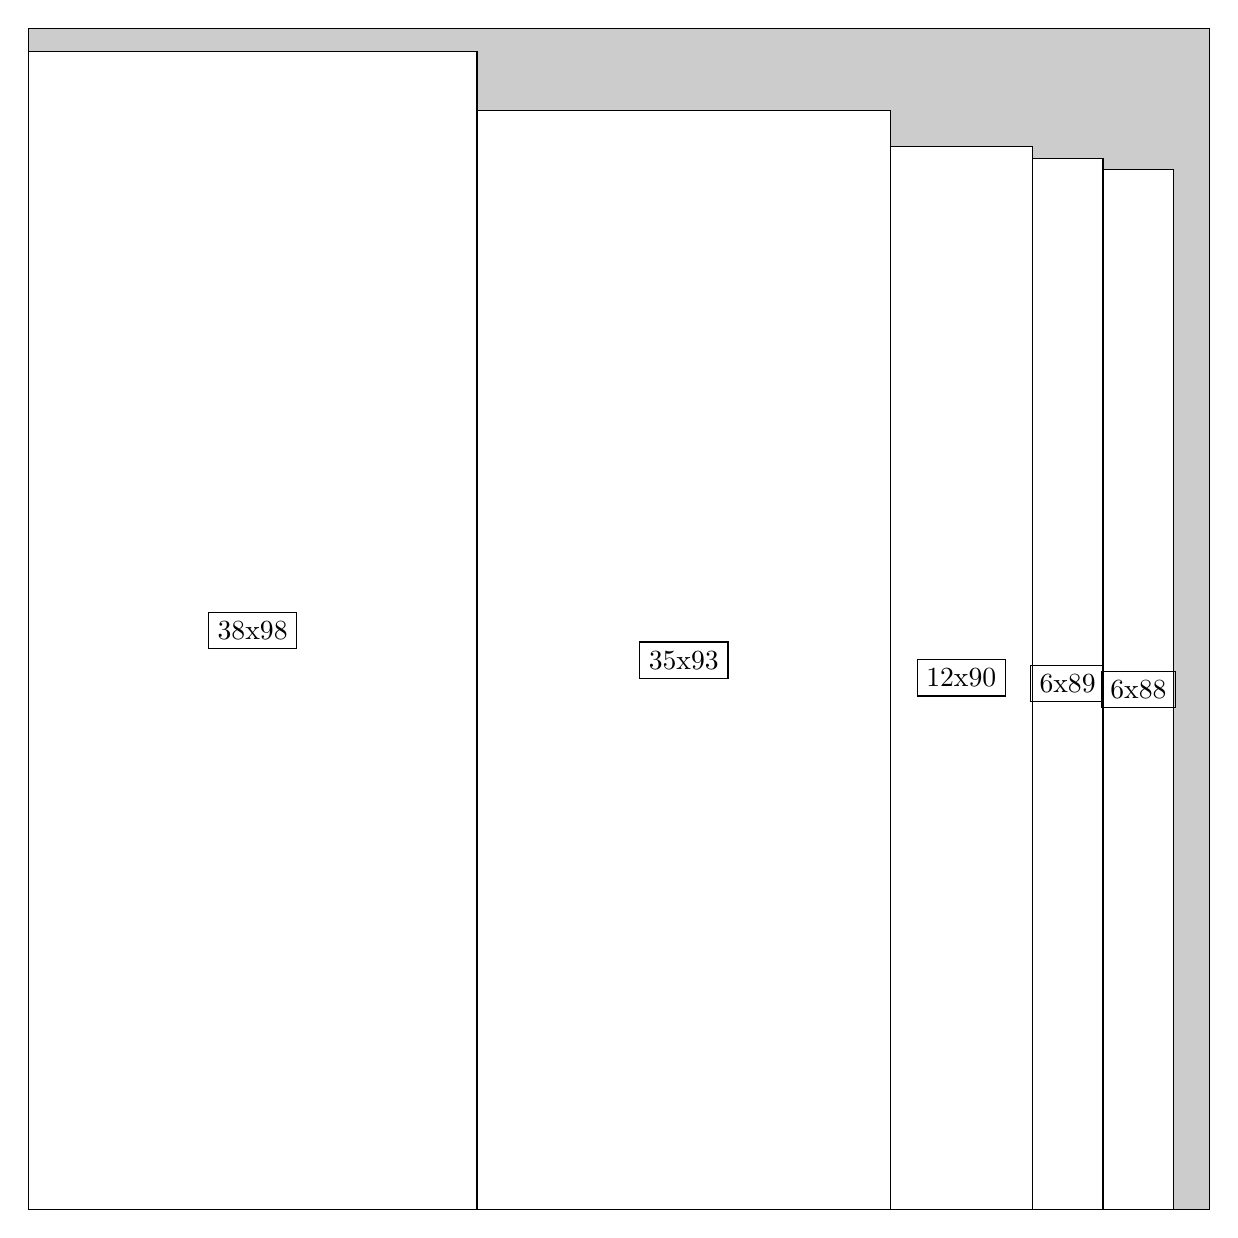
\begin{tikzpicture}[shorten >=1pt,scale=1.0,every node/.style={scale=1.0},->]
\tikzstyle{vertex}=[circle,fill=black!25,minimum size=14pt,inner sep=0pt]
\filldraw[fill=gray!40!white, draw=black] (0,0) rectangle (15.0,15.0);
\foreach \name/\x/\y/\w/\h in {38x98/0.0/0.0/5.7/14.7,35x93/5.7/0.0/5.25/13.95,12x90/10.95/0.0/1.7999999999999998/13.5,6x89/12.75/0.0/0.8999999999999999/13.35,6x88/13.65/0.0/0.8999999999999999/13.2}
\filldraw[fill=white!40!white, draw=black] (\x,\y) rectangle node[draw] (\name) {\name} ++(\w,\h);
\end{tikzpicture}


w =38 , h =98 , x =0 , y =0 , v =3724
\par
w =35 , h =93 , x =38 , y =0 , v =3255
\par
w =12 , h =90 , x =73 , y =0 , v =1080
\par
w =6 , h =89 , x =85 , y =0 , v =534
\par
w =6 , h =88 , x =91 , y =0 , v =528
\par
\newpage


\end{document}